\hypertarget{ch:data}{%
\chapter{Data Collection and Selection Bias}\label{ch:data}}

\begin{example}[The 1936 Literary Digest Poll]
  \begin{itemize}
  \item For the 1936 presidential election, the Literary Digest predicted that Alfred Landon would get 57\% of the vote against Franklin D. Roosevelt's 43\%, while the actual results were 62\% for Roosevelt against 38\% for Landon.
  \item The Literary Digest poll was one of the largest and most expensive polls with a sample size of around 2.4 million people!
  \item At the same time, George Gallup was able to predict a victory for Roosevelt using a much smaller sample of about 50,000 people.
  \item Literary Digest's sampling method: Based on every telephone directory in the United States, lists of magazine subscribers, rosters of clubs and associations, and other sources, a mailing list of about 10 million names was created. Every name on this lest was mailed a mock ballot and asked to return the marked ballot to the magazine.
  \end{itemize}
  {
    \color{red} Discuss the two problems of Literry Digest Poll. 
  }
  % The presidential election of 1936 pitted Alfred Landon, the Republican governor of Kansas, against the incumbent President, Franklin D. Roosevelt. The year 1936 marked the end of the Great Depression, and economic issues such as unemployment and government spending were the dominant themes of the campaign. The Literary Digest was one of the most respected magazines of the time and had a history of accurately predicting the winners of presidential elections that dated back to 1916. For the 1936 election, the Literary Digest prediction was that Landon would get 57\% of the vote against Roosevelt's 43\% (these are the statistics that the poll measured). The actual results of the election were 62\% for Roosevelt against 38\% for Landon (these were the parameters the poll was trying to measure). The sampling error in the Literary Digest poll was a whopping 19\%, the largest ever in a major public opinion poll. Practically all of the sampling error was the result of sample bias.

% The irony of the situation was that the Literary Digest poll was also one of the largest and most expensive polls ever conducted, with a sample size of around 2.4 million people! At the same time the Literary Digest was making its fateful mistake, George Gallup was able to predict a victory for Roosevelt using a much smaller sample of about 50,000 people.
\end{example}

\hypertarget{data}{%
\section{Berkson's bias}\label{berkson-bias}}

The following impressions are common, but are then really true?
  \begin{itemize}
  \item Hollywood ruins good books.
    \begin{itemize}
    \item \href{https://www.yardbarker.com/entertainment/articles/popular_books_that_were_made_into_terrible_movies/s1__29971472}{Popular books that were made into terrible movies}
    \item \href{https://www.cinelinx.com/movie-news/movie-stuff/bad-books-that-made-great-films/}{Bad Books That Made Great Films} 
    \end{itemize}
  \item Handsome men are such jerks.
  \item More talented people are less attractive.
  \item Smarter students spend less time on studying. 
  \item The list can go on forever ...
  \end{itemize}
% Consider a retrospective study examining a risk factor for a disease. If samples are taken from a hospital in-patient population, rather than from the general public, this can result in a spurious negative association between the disease and the risk factor. For example, if the risk factor is diabetes and the disease is cholecystitis, a hospital patient without diabetes may be more likely to have cholecystitis than a member of the general population. This is because the patient must have had some non-diabetes (possibly cholecystitis-causing) reason to enter the hospital in the first place. That result will be obtained regardless of whether there is any association between diabetes and cholecystitis in the general population.
The impressions listed above are obtained based biased data related to Berkson's bias. Let's start with an example to explain. 
\begin{example}[Stumps display]
  Suppose you have 1000 postage stamps: 300 are pretty, 100 are rare, and 30 are both pretty and rare. Is a rare stamp more likely to be pretty? 
Now you want to show some of your stamps to your friends, you probably want to show them the pretty ones and the rare ones. Lets say you only show the 370 stamps which are either pretty or rare to your friends. Based on what your friends observed, will they conclude that a rare stamp more likely to be pretty?
\end{example}

Let's calculate the numbers now: For all the stamps, the probability that a stamp is pretty is 300/1000=0.3; for rare stamps, the probability that a stamp is pretty is 30/100=0.3. A rare stamp is not more likely to be pretty.

For the stamps your friends saw, the probability that a stamp is pretty is 300/370=0.81; for rare stamps, the probability that a stamp is pretty is 30/100=0.3. Your friends' conclusion: a rare stamp is much less likely to be pretty!

The reason for their incorrect conclusion is that the 370 stumps are not a representative sample of all the stamps you have. The sample is biased.

% 10\% of all his stamps are rare and 10\% of his pretty stamps are rare, so prettiness tells nothing about rarity. He puts the 370 stamps which are pretty or rare on display. Just over 27\% of the stamps on display are rare (100/370), but still only 10\% of the pretty stamps are rare (and 100\% of the 70 not-pretty stamps on display are rare). If an observer only considers stamps on display, they will observe a spurious negative relationship between prettiness and rarity as a result of the selection bias (that is, not-prettiness strongly indicates rarity in the display, but not in the total collection).
Now let's simulate some data to further illustrate.

\input{Rnw/datacollect-Berkson}

\hypertarget{data}{%
\section{Survival Bias}\label{survival-bias}}
During World War II, aircraft that had returned from missions were examined and  the most-hit areas of the plane are given in Figure~\ref{fig:survival-bias}. Which areas should the army add armor to increase the survivorship of the planes? A direct intuition may suggest to reinforce areas with the most bullet holes. However, this is not a wise decision. Why? The data were collected from the aircraft that had survived their missions so they are biased. Planes that had been shot down or otherwise lost had not been counted. The bullet holes in the returning aircraft represented areas where a plane could take damage and still fly well enough to return safely. Thus, it is the areas where the returning aircraft were unscathed that need additional armor. 

% the statistician Abraham Wald took survivorship bias into his calculations when considering how to minimize bomber losses to enemy fire.[11] The Statistical Research Group (SRG) at Columbia University, which Wald was a part of, examined the damage done to aircraft that had returned from missions and recommended adding armor to the areas that showed the least damage, based on his reasoning.
% This contradicted the US military's conclusions that the most-hit areas of the plane needed additional armor.[12][13][14] Wald noted that the military only considered the aircraft that had survived their missions; any bombers that had been shot down or otherwise lost had logically also been rendered unavailable for assessment. The bullet holes in the returning aircraft, then, represented areas where a bomber could take damage and still fly well enough to return safely to base. Thus, Wald proposed that the Navy reinforce areas where the returning aircraft were unscathed,[11]:88 since those were the areas that, if hit, would cause the plane to be lost. His work is considered seminal in the then-nascent discipline of operational research.[15]

\begin{figure}
  \centering
  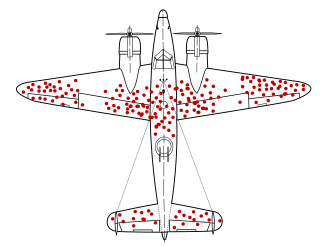
\includegraphics[width=\textwidth]{images/Survivorship-bias.png}
  \caption{Most-hit areas of the returned aircraft}
  \label{fig:survival-bias}
\end{figure}

\hypertarget{data}{%
  \section{Common sources of biases}\label{sources-bias}}
\begin{itemize}
\item Observation time interval: 
Early termination of a trial at a time when its results support the desired conclusion.
\item Data partition: divide data with knowledge of the contents of the partitions. 
\item Confirmation bias: to search for, interpret, favor, and recall information in a way that confirms or supports one's prior beliefs or values. A famous is cherry picking. % The term is based on the perceived process of harvesting fruit, such as cherries.
  The picker would be expected to select only the ripest and healthiest fruits. An observer who sees only the selected fruit may thus wrongly conclude that most, or even all, of the tree's fruit is in a likewise good condition.
\item Rejection of bad data on (1) arbitrary grounds, instead of according to previously stated or generally agreed criteria or (2) discarding "outliers" on statistical grounds that fail to take into account important information that could be derived from "wild" observations.
\item Self-selection bias or a volunteer bias.  % in studies offer further threats to the validity of a study as these participants may have intrinsically different characteristics from the target population of the study. Studies have shown that volunteers tend to come from a higher social standing than from a lower socio-economic background.[20] Further, to this another study shows that women are more probable to volunteer for studies than males. Volunteer bias is evident throughout the study life-cycle, from recruitment to follow-ups. More generally speaking volunteer response can be put down to individual altruism, a desire for approval, personal relation to the study topic and other reasons.[20][14] As with most instances mitigation in the case of volunteer bias is an increased sample size.[c
\item Nonresponse bias: It is often related to sensitive questions.
\item Rejection of bad data on (1) arbitrary grounds, instead of according to previously stated criteria or (2) discarding ``outliers'' on statistical grounds that fail to take into account important information that could be derived from ``wild'' observations.
\item Length time bias: It often occurs in cancer screening studies. Compared with fast-growing tumors, slow-growing tumors has a longer period of time during which the cancer is in the body but not large enough to cause symptoms. Thus if the same number of slow-growing and fast-growing tumors appear in a year, the screening test detects more slow-growers than fast-growers. If the slow growing tumors are less likely to be fatal than the fast growers, the people whose cancer is detected by screening do better, on average, than the people whose tumors are detected from symptoms. This may give the impression that detecting cancers by screening causes cancers to be less dangerous.  % even if less dangerous cancers are simply more likely to be detected by screening.[1]

\end{itemize}

\hypertarget{data}{%
  \section{Some basic sampling designs}\label{sampling-designs}}
  \begin{itemize}
  \item Simple Random Sampling: Every elements in the target population have equal chances to be selection. Samples are selected strictly by chance. It is probably the most effective method to prevent sampling bias. A disadvantage is the uncertainty may be large.
  \item Stratified Sampling: Divide members of the population into homogeneous subgroups and then use simple random sampling for each subgroups. It helps to reduce the uncertainty. Need to be careful of potential biases.
  \item Weighted Sampling: Let more informative elements have higher chances to be selected. It may increase the estimation efficiency, but the resulting sample may be biased so need special way of estimation.
  \end{itemize}
\hypertarget{data}{%
  \section{Different sampling approaches}\label{sampling-approaches}}
%%%%----------------------------------------------------------
  \begin{itemize}
  \item Sampling with replacement: An element may be included in a sample more than once. It is possible to have replicates in the sample.
  \item Sampling without replacement: An element can be included in a sample at most once. There is no replicates in the sample.
  \item Poisson sampling: determines if each element of the population is selected in the sample independently. The sample size is random.
  \item Between Sampling with replacement and without replacement, which is more efficient?
  \end{itemize}
%%%%----------------------------------------------------------
\begin{example}[Numerical comparisons]
  \begin{itemize}
  \item To simulation hosehold incomes, generate a population P of size $N$ from a $P\sim\chi^2$ distribution with degrees of freedom one.
  \item Take samples of size $n$ from P to estimator the population mean, say $\mu$, using simple random sampling both with and without replacement. Compare their efficiency.
  \item Assume another variable $A=P+Unif(0,2)$ is available to define informative sampling weights. Evaluate the efficiency of weighted sampling both with and without replacement. 
  \end{itemize}
\end{example}
%%% Local Variables:
%%% coding: utf-8
%%% mode: latex
%%% TeX-master: "00why.tex"
%%% End:

%%% TeX-engine: xetex
%%% TeX-command-extra-options: "-shell-escape"
